\documentclass[11pt, letterpaper]{article}
\input{../../homework.tex}
\usepackage{titlepageBU}
\title{Problem Set 10}
\courseID{PY 451}
\courseSection{A1}
\usepackage{mleftright}
\renewcommand{\left}{\mleft}
\renewcommand{\right}{\mright}
\begin{document}
\makeproblem
\section{Scattering}
\begin{enumerate}
	\item 
		\begin{lstlisting}[language=mathematica]
haiiii:=1.60218*10^(-16) (* conversion keV -> J *)
e := 10^(-18) * haiiii (* keV *)
m := 9.1093837139*10^(-31) (*kg*)
hbar:=1.054571817*10^(-34)  (*J s*)
a:=0.01 (*m*)

V0[Y_]:=10^(-18)*Y*haiiii

k1:=Sqrt[ (2*m*e)/(hbar^2)]
k2[Y_]:=Sqrt[(2*m*(e+V0[Y]))/(hbar^2)]

T[Y_]:=1/(1+(((k1^2-k2[Y]^2)^2*(Sin[2*k2[Y]*a])^2)/(4*k1^2*k2[Y]^2)))
Plot[
  T[Y],
  {Y, -10, 4},
  PlotRange -> All,
  AxesLabel -> {"Y (keV)", "T"},
  PlotLabel  -> "Transmission vs. Barrier Height Y"
]
		\end{lstlisting}
		Output:
		\begin{figure}[ht]
			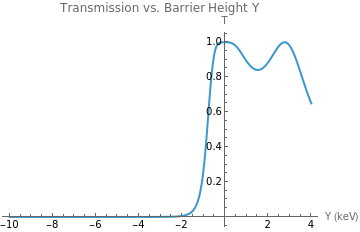
\includegraphics{../figures/owo.png}
		\end{figure}
		The equation peaks at 1 twice, around $Y=0$ and $Y=2.3$. It's also basically 0 until $Y=-2$, at which point it shoots up. After attaining it's final peak, it goes down.
	\item No thanks
\end{enumerate}


\section{3d Wavefunctions}
\begin{enumerate}
	\item Note - when I switched all the integrals into cylindrical coordinates, I used $\theta $ as the variable instead of $\varphi $ because I forgot we were using $\theta $ as the step function. Because of this, all of my integrals use $\theta $ as a function AND as the variable to be integrated on. I can't be asked fixing the notation, and either way it should be clear when $\theta $ is the step function and when it is the variable. Because $\left| e^{i\theta }  \right| =1$, and since we clearly have $\left| \theta (x) \right| ^2=\theta (x)$ since $\theta $ can only equal 0 or 1, we have
		\begin{align*}
			\braket{\psi }{\psi } &=\iiint\limits_{\mathbb{R} ^3} A^2\left| e^{-z^2/a^2} \theta \left( b^2-\left( x^2+y^2 \right)  \right)  \right| ^2 \,\mathrm{d}\mu   \\
					      &=A^2 \int_{-\infty }^{\infty }\int_{-\infty }^{\infty } \theta \left( b^2-\left( x^2+y^2 \right)  \right) \int_{-\infty }^{\infty } \left( e^{-z^2/a^2} \right)^2  \,\mathrm{d} z\mathrm{d} y \mathrm{d} x\\
					      &=A^2\int_{-\infty }^{\infty }\int_{-\infty }^{\infty } \theta \left( b^2-\left( x^2 +y^2\right)  \right) \int_{-\infty }^{\infty } e^{-z^2\left( 2/a^2 \right)  }  \,\mathrm{d} z\mathrm{d} y \mathrm{d} x\\
					      &\text{Let } u=z\frac{\sqrt{2}}{a} \\
					      &=A^2\int_{-\infty }^{\infty }\int_{-\infty }^{\infty } \theta \left( b^2-\left( x^2+y^2 \right)  \right) \int_{-\infty }^{\infty } \frac{a}{\sqrt{2}} e^{-u^2}  \,\mathrm{d} u\mathrm{d} y \mathrm{d} x\\
					      &=A^2a \sqrt{\frac{\pi }{2} } \int_{-\infty }^{\infty }\int_{-\infty }^{\infty } \theta \left( b^2-\left( x^2+y^2 \right)  \right)  \,\mathrm{d} y \mathrm{d} x\\
					      &=A^2a \sqrt{\frac{\pi }{2} } \int_{0}^{2\pi }\int_{0}^{\infty } \theta \left( b^2-r^2 \right) r \,\mathrm{d} r \mathrm{d} \theta \\
					      &=A^2a \sqrt{\frac{\pi }{2} } \int_{0}^{2\pi }\int_{0}^{\left| b \right| } r \,\mathrm{d} r \mathrm{d} \theta +A^2a \sqrt{\frac{\pi }{2} } \int_{0}^{2\pi }\int_{\left| b \right| }^{\infty } 0 \,\mathrm{d} r \mathrm{d} \theta \\
					      &=A^2a\sqrt{\frac{\pi }{2} } \pi b^2\\
					      &=\frac{A^2ab^2\sqrt{\pi ^3} }{\sqrt{2} } \\
					      &\equiv 1	
		,\end{align*}
		where I have set $\theta ^2=\theta $ due to the fact that
		\[
			\theta \left( b^2-r^2 \right) =
			\begin{cases}
				1,&\left| b \right| \geq \left| r \right| \\
				0,&\left| b \right| <\left| r \right| 
			\end{cases}
		.\]
		It follows that
		\[
			A=\sqrt{\frac{\sqrt{2} }{ab^2\sqrt{\pi ^3} } } 
		.\]
	\item First, we compute the partial derivatives
		\[
			\frac{\partial \psi }{\partial x} =Ae^{-z^2/a^2}  e^{i(p_xx+p_yy) /\hbar }\left( \frac{ip_x}{\hbar } \theta \left( b^2-\left( x^2+y^2 \right)  \right) -2x\delta \left( b^2-\left( x^2+y^2 \right)  \right)  \right) 
		,\]
		\[
			\frac{\partial \psi }{\partial y} =Ae^{-z^2/a^2}  e^{i(p_xx+p_yy) /\hbar }\left( \frac{ip_y}{\hbar } \theta \left( b^2-\left( x^2+y^2 \right)  \right) -2y\delta \left( b^2-\left( x^2+y^2 \right)  \right)  \right) 
		.\]
		For simplicity, denote by $\phi $ the exponential stuff outside of the parenthases. The notation $\phi (x)$ should be interpreted as ``$\phi \times x$'', not as inserting $x$ into the function $\phi $. In other words, just interpret it as a constant, as I will expand it out any time we actually need to work with the stuff inside of it. We then have
		\[
			\partial_x \psi =\phi \left( \frac{ip_x}{\hbar } \theta -2x\theta ' \right) ,\qquad \partial_y \psi =\phi \left( \frac{ip_y}{\hbar } \theta -2y\theta ' \right) 
		,\]
		with the implied arguments for the function $\theta $. We then have
		\[
			\left( XP_y-YP_x \right)\psi  =\left( -i\hbar x \partial_y+i\hbar y \partial _x \right) \psi =i\hbar \phi \left( 2xy\theta '-2xy\theta '-\frac{ixp_y}{\hbar } \theta +\frac{iyp_x}{\hbar } \theta  \right) =\phi (xp_y-yp_x)\theta 
		.\]
		Therefore, $\bra{\psi } \left( XP_y-YP_x \right) \ket{\psi } $ equals the following.
		\begin{align*}
			&\int_{-\infty }^{\infty }\int_{-\infty }^{\infty }\int_{-\infty }^{\infty } \phi^2\theta \left( b^2-\left( x^2+y^2\right)  \right) \left( xp_y-yp_x \right) \theta \left( b^2-\left( x^2+y^2 \right)  \right)  \,\mathrm{d} z \mathrm{d} y \mathrm{d} x\\
			&=A^2\int_{0}^{2\pi}\int_{0}^{\infty }\int_{-\infty }^{\infty } e^{-z^2(2/a^2)} \theta \left( b^2-r^2  \right) \left( p_y r \cos \theta - p_x r \sin \theta  \right)  r\,\mathrm{d} z \mathrm{d} r\mathrm{d} \theta \\
			&=A^2a \sqrt{\frac{\pi }{2} } \int_{0}^{2\pi }\int_{0}^{\infty }r^2 \theta \left( b^2-r^2 \right) \left( p_y\cos \theta -p_x\sin \theta  \right)  \,\mathrm{d} r \mathrm{d} \theta \\
			&=A^2a\sqrt{\frac{\pi }{2} } \int_{0}^{2\pi }\int_{0}^{\left| b \right| } r^2\left( p_y \cos \theta -p_x \sin \theta  \right)  \,\mathrm{d} r \mathrm{d} \theta \\
			&=A^2 a \sqrt{\frac{\pi }{2} } \int_{0}^{2\pi } \frac{\left| b \right| ^3}{3} \left( p_y \cos \theta - p_x \sin \theta  \right)  \,\mathrm{d} \theta \\
			&=\frac{A^2 a\left| b \right| ^3}{3} \sqrt{\frac{\pi }{2} } p_y(1-1)\\
			&=0
		.\end{align*}
	\item Reusing our result from part 2, we have
		\[
			\left( XP_y-YP_x \right) \psi =\phi \left( xp_y-yp_x \right) \theta
		,\]
		once again with implied arguments for $\theta $ to simplify notation. We now want to find
		\[
			\left( XP_y-YP_x \right) \left( \phi \left( xp_y-yp_x \right) \theta  \right) 
		.\]
		Note that
		\[
			\frac{\partial }{\partial x} \left( xp_y-yp_x \right)\theta =p_y\theta -2x\left( xp_y-yp_x \right) \theta '
		.\]
		Also note that
		\[
			\frac{\partial }{\partial x} \phi =\frac{ip_x}{\hbar } \phi 
		.\]
		We thus have
		\[
			\frac{\partial }{\partial x} \left( \phi \left( xp_y-yp_x \right) \theta  \right) =\frac{ip_x}{\hbar } \phi\left( xp_y-yp_x \right) \theta +\phi p_y\theta -2x\phi \left( xp_y-yp_x \right) \theta '
		.\]
		By analogous logic,
		\[
			\frac{\partial }{\partial y} \left( \phi \left( xp_y-yp_x \right) \theta  \right) =\frac{ip_y}{\hbar } \phi \left( xp_y-yp_x \right) \theta -\phi p_x\theta -2y\phi \left( xp_y-yp_x \right) \theta '
		.\]
		Multiplying through by $y$ and $x$ respectively, and subtracting,  we obtain
		\[
			\frac{ixp_y}{\hbar } \phi \left( xp_y-yp_x \right) \theta -\phi xp_x\theta -2xy\phi \left( xp_y-yp_x \right) \theta '-\left( \frac{iyp_x}{\hbar } \phi \left( xp_y-yp_x \right) \theta +\phi yp_y\theta -2xy\phi \left( xp_y-yp_x \right) \theta ' \right) 
		\]
		\[
			=\left( \frac{i}{\hbar } \phi \left( xp_y-yp_x \right) \left( xp_y-yp_x \right) -\phi xp_x-\phi yp_y \right) \theta 
		.\]
		Multiplying through by $-i\hbar $ gives
		\[
			(XP_y-YP_x)^2\psi =\left( \phi (xp_y-yp_x)^2-i\hbar \phi \left(xp_x+yp_y \right)\right) \theta 
		.\]
		Calculating $\bra{\psi } \left( XP_y-YP_z \right)^2 \ket{\psi } $ gives
		\begin{align*}
			&\;\;\;\; \int_{-\infty }^{\infty }\int_{-\infty }^{\infty }\int_{-\infty }^{\infty } A^2e^{-z^2(2/a^2)} \theta \left( b^2-\left( x^2+y^2 \right)  \right) \left(\left( xp_y-yp_x \right) ^2-i\hbar \left( xp_x+yp_y \right)\right)  \,\mathrm{d} z \mathrm{d} y \mathrm{d} x\\
			&=A^2a\sqrt{\frac{\pi }{2} } \int_{0}^{2\pi }\int_{0}^{\infty } \theta \left( b^2-r^2 \right) \left( r^2 p^2_y \cos ^2\theta +r^2p^2_x \sin ^2\theta -2rp_xp_y \cos \theta \sin \theta -ri\hbar \left( p_x \cos \theta +p_y \sin \theta  \right)  \right) r \,\mathrm{d} r \mathrm{d} \theta \\
			&=A^2a\sqrt{\frac{\pi }{2} } \int_{0}^{2\pi }\int_{0}^{\left| b \right|} r^3 p^2_y \cos ^2\theta +r^3p^2_x \sin ^2\theta -2r^2p_xp_y \cos \theta \sin \theta -r^2i\hbar \left( p_x \cos \theta +p_y \sin \theta  \right) \,\mathrm{d} r \mathrm{d} \theta \\
			&=A^2a\sqrt{\frac{\pi }{2} } \int_{0}^{2\pi } \frac{b^4}{4} p_y^2 \cos ^2\theta +\frac{b^4}{4} p_x^2 \sin ^2\theta -2\frac{\left| b \right| ^3}{3} p_xp_y \cos \theta \sin \theta -\frac{\left| b \right|^3}{3} i\hbar \left( p_x \cos \theta +p_y \sin \theta  \right)  \,\mathrm{d} \theta \\
			&=A^2 a \sqrt{\frac{\pi }{2} } \int_{0}^{2\pi } \frac{b^4p_y^2}{8} \left( \cos 2\theta +1 \right) +\frac{b^4p_x^2}{8} \left( 1-\cos 2\theta  \right) -\frac{\left| b \right| ^3p_xp_y}{3} \sin 2\theta -\frac{\left| b \right| ^3i\hbar }{3} \left( p_x \cos \theta +p_y \sin \theta  \right)  \,\mathrm{d} \theta \\
			&=A^2a\sqrt{\frac{\pi }{2} } \left( -\frac{\left| b \right| ^3i\hbar }{3} \left( p_x \cos \theta +p_y \sin \theta  \right)_0^{2\pi } +\frac{1}{2} \int_{0}^{4\pi } \frac{b^4p_y^2}{8} (\cos \theta +1)+\frac{b^4p_x^2}{8} (1-\cos \theta )-\frac{\left| b \right| ^3p_xp_y}{3} \sin \theta  \,\mathrm{d} \theta  \right) \\
			&=\frac{A^2a}{2} \sqrt{\frac{\pi }{2} } \int_{0}^{4\pi } \frac{b^4p_y^2}{8} \cos \theta -\frac{b^4p_x^2}{8} \cos \theta -\frac{\left| b \right| ^3p_xp_y}{3} \sin \theta  \,\mathrm{d} \theta +\frac{A^2a}{2} \sqrt{\frac{\pi }{2} } \left( \frac{b^4p_y^2 \pi }{2} +\frac{b^4p_x^2\pi }{2}  \right) \\
			&=\frac{A^2ab^4\pi }{4} \sqrt{\frac{\pi }{2} } \left( p_x^2+p_y^2 \right) 
		.\end{align*}
\end{enumerate}

\end{document}
